% !TeX root = ../main.tex

\chapter{绪论}

\section{研究背景}
为了进一步加深对宏观实验结果的认识,探索微观体系就成了一种不可或缺的途径。例如,对特定都进不了在催化过程中可能存在的不同构象的模拟研究,合金以及复合材料在不同状态和比例下的性能表现。在对微观体系的探索中,主要被关注的部分则是微观粒子的运动轨迹和状态,通过对不同微观粒子在整个体系中的状态变化情况来进一步验证宏观实验现象。并且对于微观体系,可以使用周期性边界条件对粒子进行周期性扩展。这样做不仅在一定程度上扩展了规模,并且也可以规避边界效应所带来的影响。

为了进一步对微观体系进行模拟,在数十年中发展除了多种原子层面的模拟方法,其中包括分子动力学模拟,蒙特卡洛方法\cite{raychaudhuri2008introduction,bird1981monte},第一性原理方法\cite{warshel1976theoretical},晶体力学等。蒙特卡洛方法是较早出现的一种模拟方法,由于其对随机选择的步骤是接受或拒绝对基于良好的指定概率,则可以在一定体系内实现对不同能量的计算。分子动力学模拟则是通过不同体系中原子势的算法,建立由不同粒子信息所构成的模拟体系,并动态计算不同粒子的特性,包括位置信息,温度信息等,除此之外也可以计算粒子在不同状态下的微观特性。第一性原理方法则是通过密度泛函理论,结合多个原子参数,包括原子结构常数,质量和带电量,电子质量和带电量,并根据原子核与电子的相互作用,进行薛定谔方程的求解,这种方法常见于计算超晶胞,界面,团簇等结构模型。

对于分子动力学模拟来说,在采用计算机模拟之前,就发现可以通过微观体系的初始条件和相互作用就可以完成微观粒子的行为,可以通过将球体作为原子,木棍作为不同原子之间的键来模拟原子及其键之间的作用和变化。分子动力学描述的基本对象是整个粒子系统,而系统中不同粒子则主要通过势函数来表示,不同的势函数对应了不同的粒子体系,而设计并使用适合的势函数可以最大化保证计算结果的正确性。

1957 年,Alder 和Wainwright\cite{alder1957phase} 的实验得出,在刚体小球系统中,在对系统整体进行逐步压缩,并且根据维里定理和系统整体的压力分布,完成了固液不同状态之间的变化计算。因为刚体小球之间缺乏直接的相互作用力,所以液体到固体的状态变化会使能量达到最大。后续进行的均匀电子系统的实验也进一步验证了粒子间作用力的情况,这个研究成果也成为了凝聚态材料微观性质的理论基础。Lennard Jones 在上世纪 20 年代就氩原子体系提出了一种基本方法,就是经典的Lennard-Jones 势\cite{jones1924determination}。1964 年,Rahman 等人在模拟氩原子的过程中\cite{rahman1964correlations},通过采用L-J 势进行微观体系的分子动力学模拟,并统计了模拟过程中的得到的粒子信息。虽然当时的计算能力不足,导致所模拟的粒子规模只有数百个,但对在分子动力学模拟中 Lennard-Jones 势发展及其他势函数的算法都产生了深远的影响。1977 年,分子动力学模拟也首先完成了生物大分子的模拟计算\cite{mccammon1977dynamics},并且逐步完成了对蛋白质折叠,生物大分子结构等过程的微观模拟。1967 年,Verlet 提出Verlet 积分算法\cite{verlet1967computer},以及邻域列表方法,并在此基础上,又发展出了蛙跳法等算法,此类方法在大规模计算的基础上进一步减小了计算量,也推动了分子动力学模拟加速发展。随着计算性能的不断提高,在经典分子动力学模拟中,又逐步引入了带修正的势函数计算,并在热力学方向的模拟中 Zhakhovskii\cite{zhakhovskii2009molecular}采用带修正的Lennard-Jones 势函数,完成了氩原子在二维圆柱汇聚激波中的不稳定性计算。

对于分子动力学模拟的起步阶段,由于计算机算力的限制,计算只能在一定的体积之内进行。这种方法必须使能量保持守恒,并且对于模拟体系与外界不产生物质和能量的交换,这种方法称为微正则系综(micro-canonical ensemble),简称为NVE,其中粒子数量,体积,能量都是同步的,这种方法在分子动力学方向应用十分广泛。在此基础上,又发展除了另外一种方法,称为正则系综(canonical ensemble),简称为 NVT,NVT 系综与能量守恒的 NVE 不同,其通过调节能量来保持稳定的温度。通过对这两种系综的利用,可以模拟统一体系下不同阶段的粒子运动状态。

 \begin{figure}[h]
  \centering
  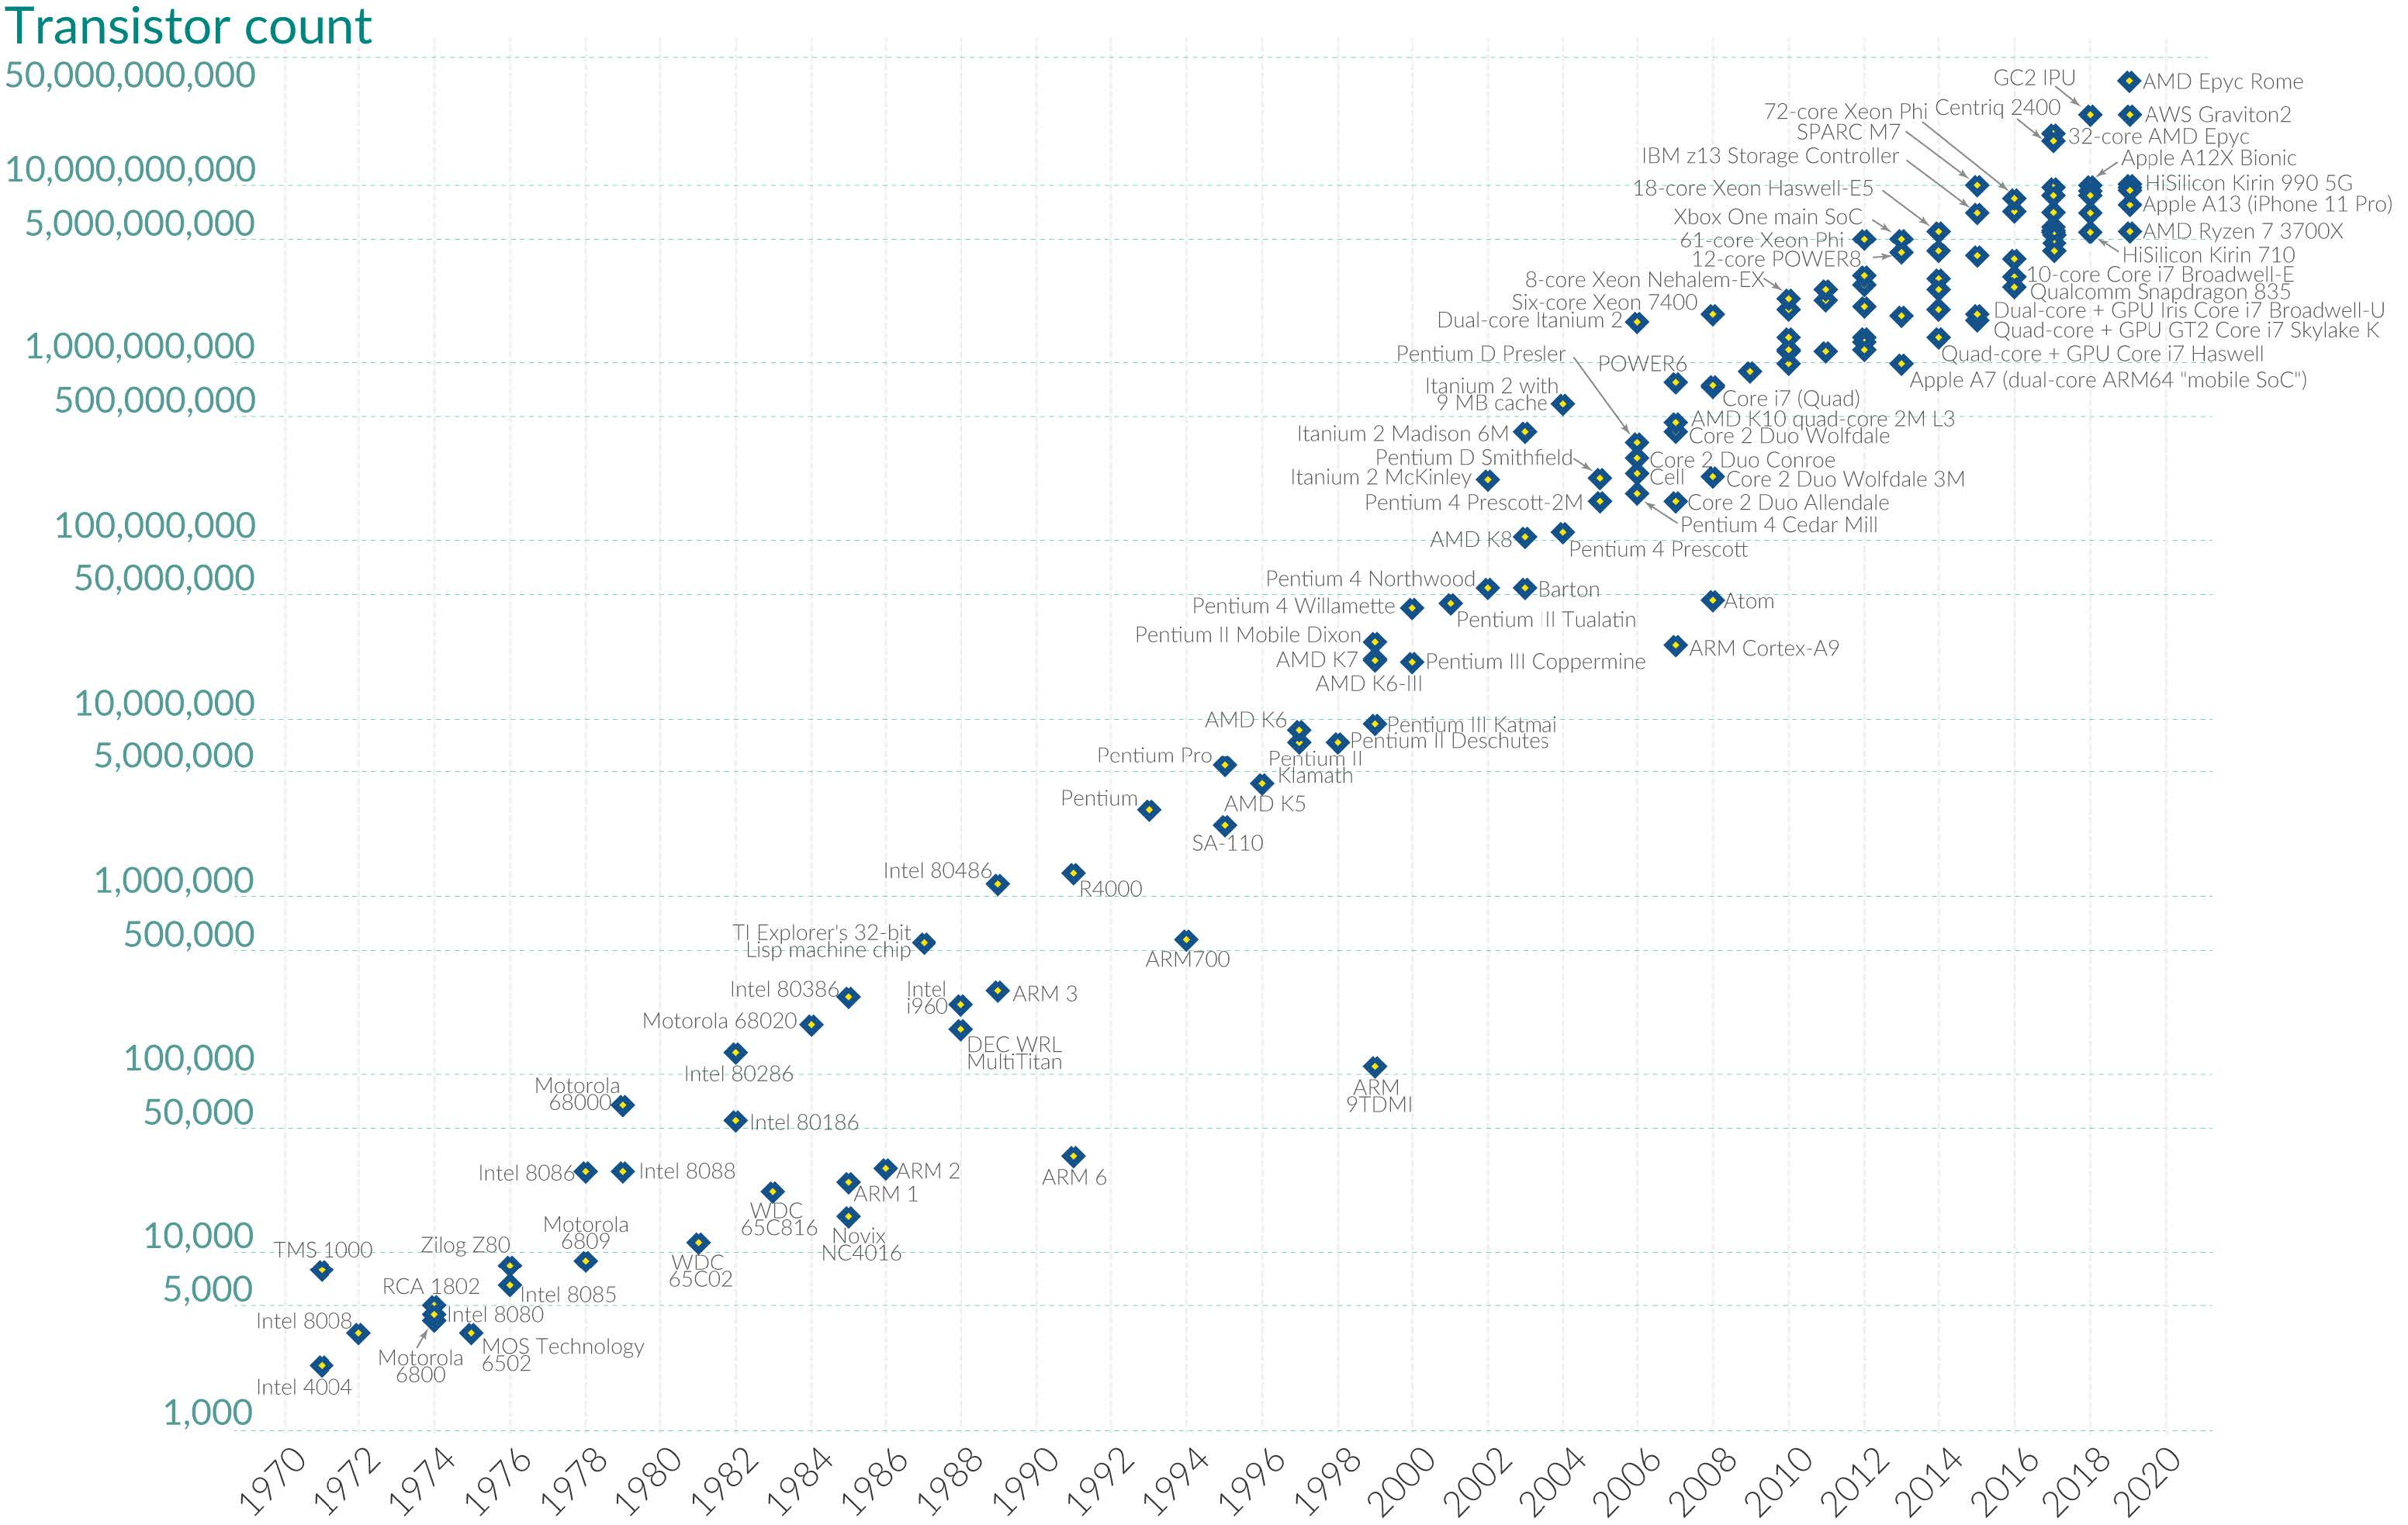
\includegraphics[width=1\textwidth]{1_1.jpg}
  \caption{微处理器中晶体管的数量增长趋势}
\end{figure}

\section{处理器发展趋势}
自从摩尔定律\cite{schaller1997moore,moore1998cramming} 第一次被提及以来,数十年间半导体技术与集成电路工艺得到了迅速的发展。在保持一定成本的前提下,以每 18 至 24 个月为时间周期,制程工艺方面的提升,使得芯片上所集成的晶体管数量和密度将提升一倍,从过去统计的数据来看,集成电路产生的成本,芯片性能都按照摩尔定律持续向前发展。但从近些年来的发展来看,这种趋势有所放缓,随着晶体管工艺的不断提升,集成电路规模不断扩大,制造工艺逐渐成为了发展的瓶颈,具体来看,物理效应和处理器功耗成为了阻碍工艺发展的两大因素。从物理方面来看,集成电路的制造工艺已经进入到介观的尺寸内,依照传统的方法,已经无法通过减小器件尺寸来保证摩尔定律的发展。至此处理器设计逐步采取在新片中封装多个处理核心来实现性能的提升。1996 年斯坦福大学首次提出了片上多处理器的概念,并首次实现多核芯片的模型。2001 年,IBM 公司首次公布了商用多核处理器Power4\cite{tendler2002power4},并且随着Intel,AMD 公司相继推出了相对应的处理器,多核处理器已经基本占据了桌面以及高性能计算等诸多领域。将多个核心同时封装在一个处理器之内,通过多线程进行任务的处理,这不仅提升了任务执行的并行性,并且由于这种多核集成的结构,使得核心间通信的延迟大幅地降低,这种多核架构也可以进行片上资源的共享,进一步提升了并行效率,这也使得多核处理器逐步发展成为了处理器市场的主流。根据核心结构的不同,多核处理器大概可分为以下两种:

\paragraph{同构多核处理器}
同构多核处理器将数个结构相同的核心进行互联,处理器核心之间具有一致的处理器结构和内部逻辑。同构多核处理器更容易进行相对完备的片上设计和布局,另一方面由于核心之间采用了相同的指令集,因此在任务并行计算以及编译器设计也是相对容易的,这样也更方便进行规模上的扩增。处理器每个核心可以相对独立地执行任务,此时每个核心功能近似于通用单核处理器,并且同构多核处理器在不同核心互联的方式与存储空间共享方面进行了单独的设计,核心之间可以通过共享存储器相连也可以通过cache 相连。这种设计也成为了市场上多核处理器的主流。由于核心设计和单核处理器类似,其核心结构较为复杂,片上能够集成的核心数量较为有限,所以核心数量至多能达到数十个左右。针对于桌面平台的处理器核心不超过 8 个,而服务器端芯片核心数量则能达到二十多个\cite{arafa2019cascade}。
\paragraph{异构多核处理器}
异构多核处理器相对于同构多核处理器最大的不同就是不同核心之间存在差异,在单个处理器中封装了多个不同类型的核心。这些核心具有不同的微架构和指令集,这种不同类型的核心可以根据特定任务的差异提供相匹配的资源和处理能力。为了满足计算任务的特定需求,在进行任务调度时,完全可以选择更为合适的核心类型进行处理,并且由于异构设计带来的计算能力之间的差异,在进行计算资源的分配时,可以利用最小的代价来匹配计算任务,异构多核处理器中有负责任务调度的主核和负责大部分计算的从核核心。再辅以进行浮点,特定计算等不同功能的核心,构成了完整的处理器。异构多核处理器中比较著名有IBM 开发的 Cell 处理器\cite{pham2005design},处理器内部包含了三类计算单元,第一类以 Power核心作为主处理器,第二类是8 个单指令多数据流向量处理器DSP,最后是一个可编程的DMA 控制器,这种设计可以使得不同处理核心之间可以共同高效完成任务负载。

随着处理器技术和体系结构的持续发展,特定领域的计算需求不断增多,多核处理器开始逐步向众核处理器进行过度。相比于多核处理器,众核处理器结构的核心数量可达到几十个以上,并且在处理器设计中多数采用了“主核心 + 协处理器”的非对称主从异构设计,众核处理器主要面向于特定领域的计算需求,提供高效的计算加速服务,并且从核核心内部结构相对简单,单核心的功耗较低,使得整体设计可以达到一个更高的效能。国产超级计算机神威·太湖之光采用了自主设计的异构众核处理器 SW26010,由于异构众核的特性,可以为特定领域的应用提供强大的计算能力。本文通过对分子动力学平台LAMMPS 的并行优化来实现申威平台上的高效计算。
\section{神威·太湖之光与申威异构众核处理器 SW26010}
\subsection{神威·太湖之光}
发布于2016 年的超级计算机神威·太湖之光\cite{fu2016sunway},是我国自主研发的首台浮点峰值性能超过十亿亿次的超级计算机系统,与其他超级计算机普遍采用通用 CPU 架构不同,它高效的计算能力源于自主研发的高性能异构众核SW26010 处理器,神威·太湖之光峰值性能可达 125PFlops,Linpack 持续性能为 93PFlops。在 2017 年 11 月发布的超级计算机 Top500 排行榜中连续第四次名列榜首,在神威·太湖之光上进行的科学计算应用“全球大气动力学隐式模拟”\cite{yang201610m} 获得高性能计算领域最高奖项“戈登·贝尔”奖。

 \begin{figure}[h]
  \centering
  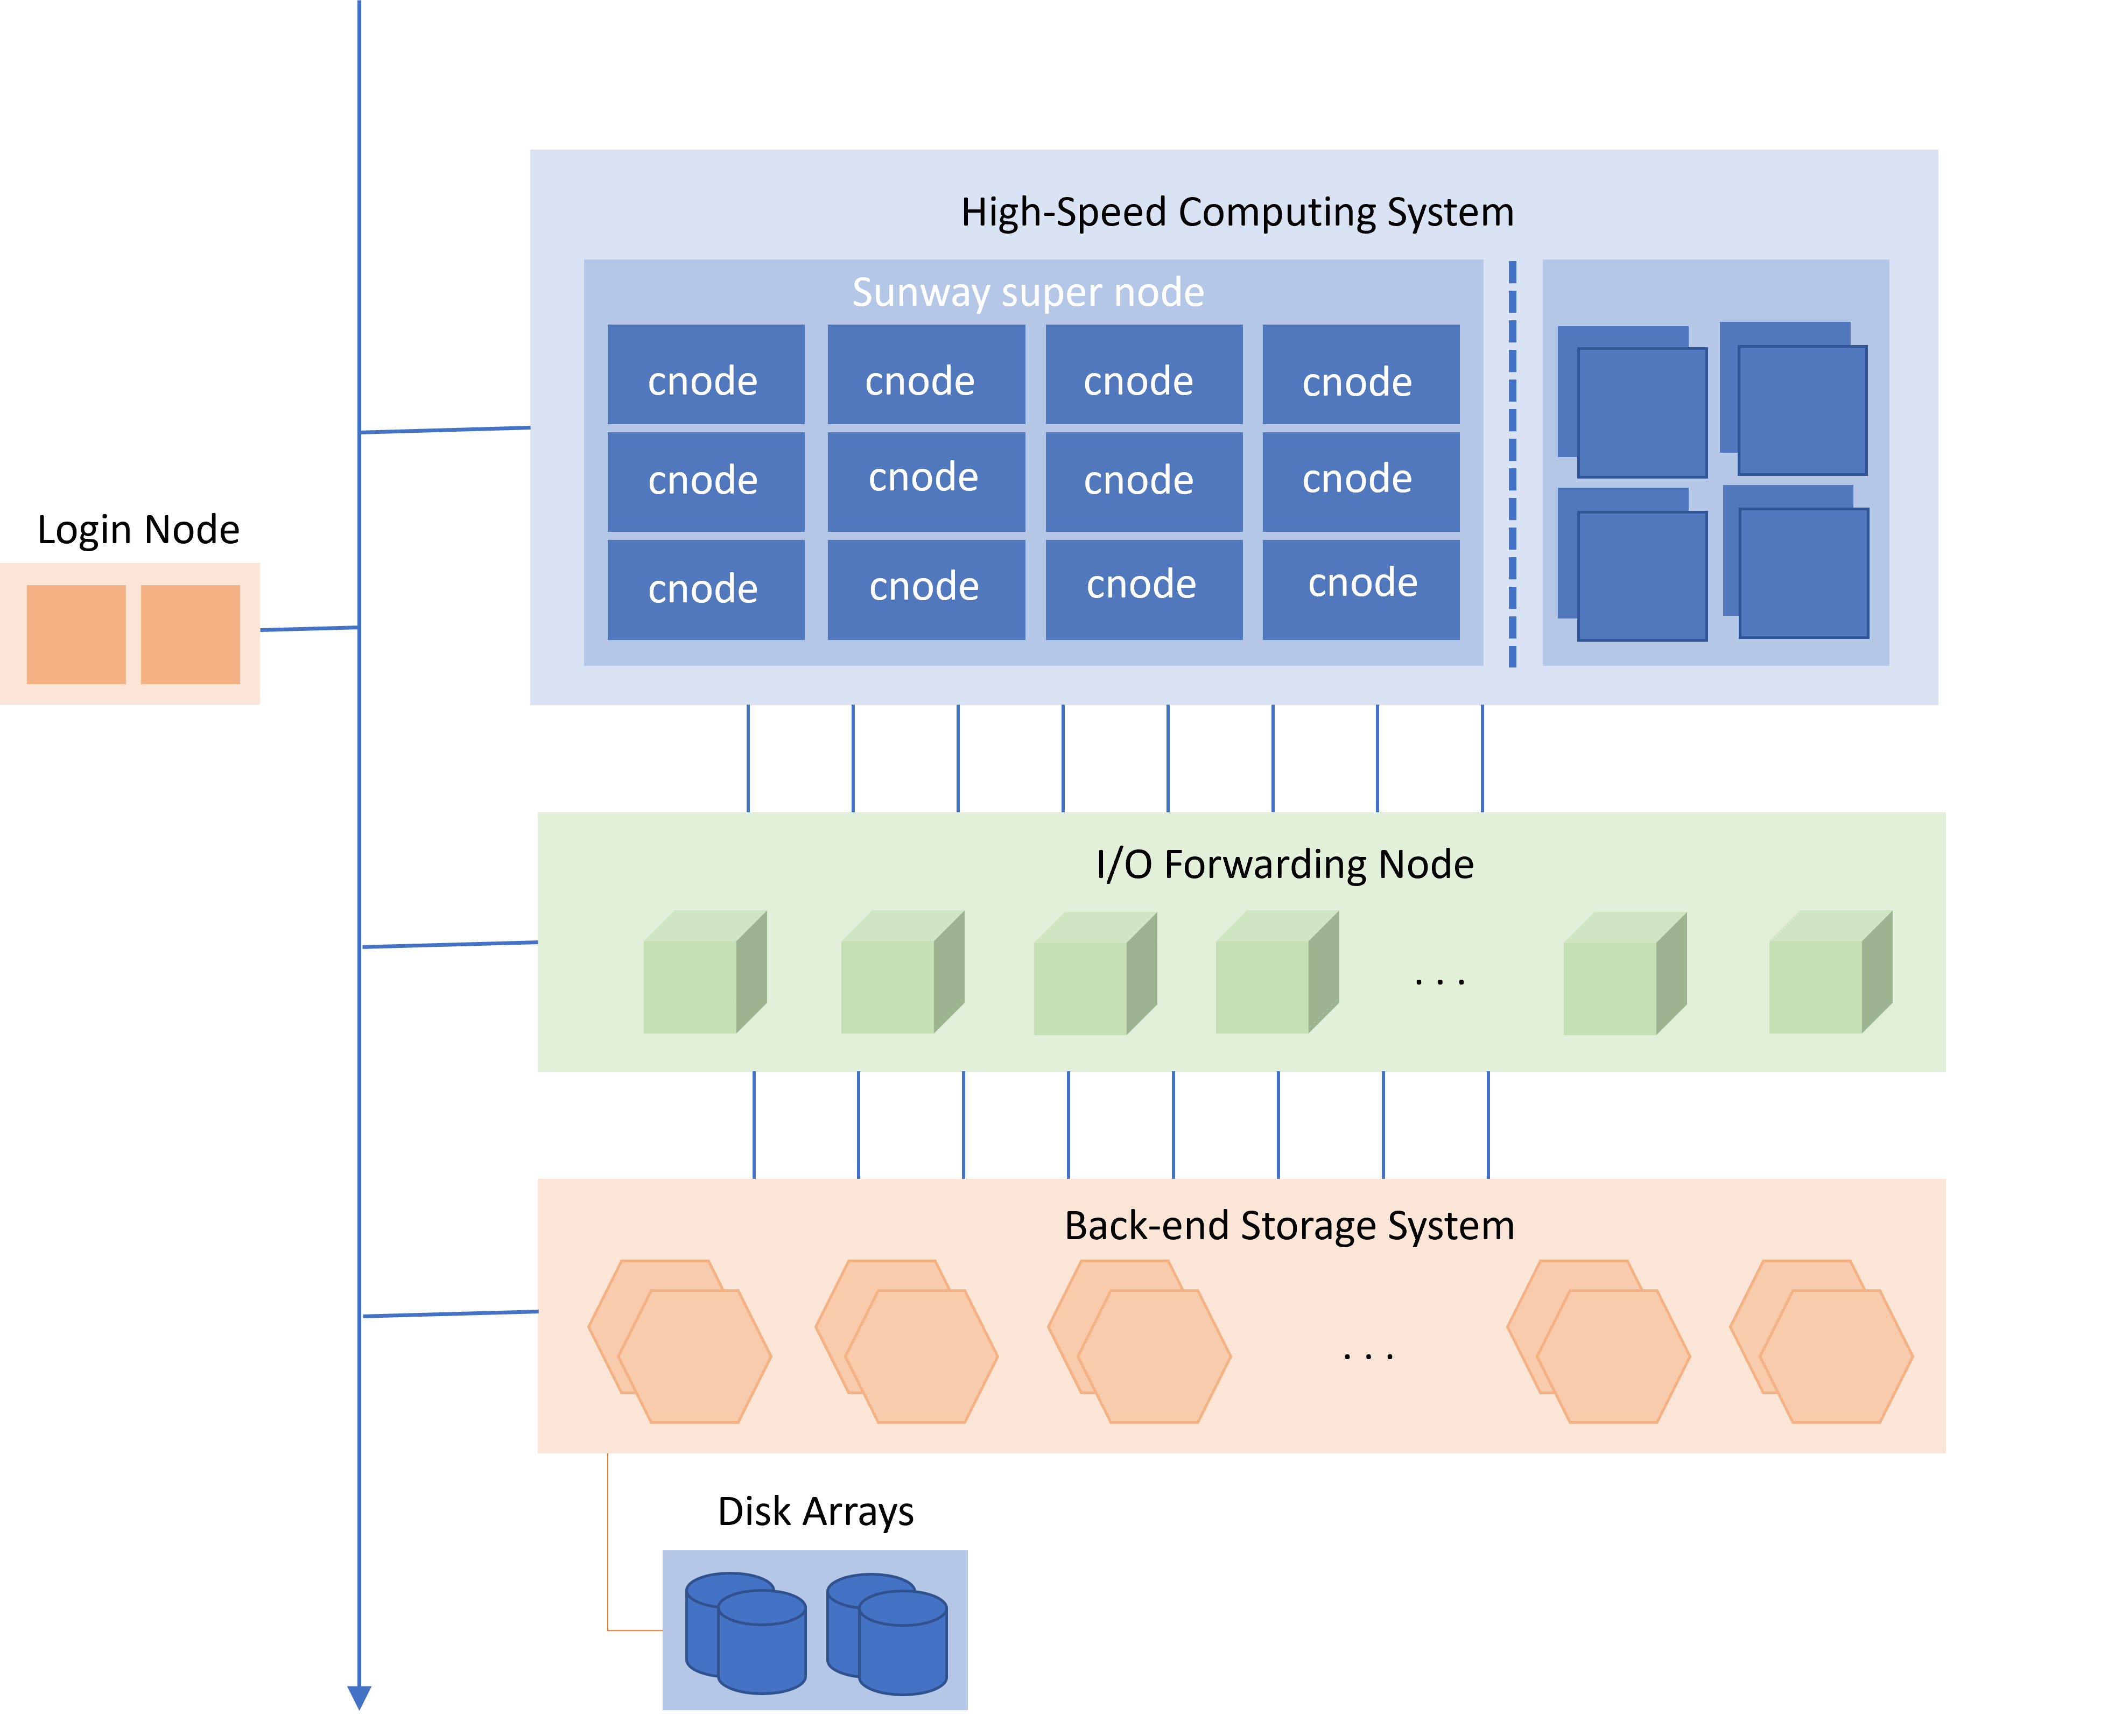
\includegraphics[width=1\textwidth]{machine.png}
  \caption{神威·太湖之光系统架构图}
\end{figure}

神威·太湖之光整机由运算系统,存储系统,管理系统等部分构成\cite{dongarra2016report},其中运算系统由 40 个机舱构成,每一个机舱包含四个超节点,每个超节点自身负责与其他超节点之间进行通信,并且支持Infiniband 通信模式。每个超节点又由256 个节点构成,节点之间由超节点支持高效的消息通信,内部采用全连接的模式。其中八个超节点构成一块插件板,每个超节点由整整 32 个插件板构成。整个网络拓扑是根据多级胖树的结构组成。存储系统负责为整个系统提供稳定的存储服务。由硬盘阵列和存储网络构成的存储系统空间大小可达 20PB。管理系统由系统控制服务器,数据库服务器构成,保证机器运算时的可靠性和稳定性。在软件系统方面,神威·太湖之光单独开发配置操作系统,高性能编译器,基础数学库,作业管理系统等环境。
\subsection{申威异构众核处理器 SW26010}
SW26010 异构众核处理器是由国家并行计算机工程技术研究中心自主研发设计的一款高性能处理器\cite{lin2018evaluating}。每块处理器共有260 个核心,集成在4 个核组中,每个核组包含 1 个主核和 64 个从核。处理器运行频率为 1.45GHz,核组之间由片上网络所联通,对于核组中的每个主核,负责运行操作系统,I/O 操作以及进行所在核组内任务的划分工作,并可以完成部分计算任务。主核内带有两条浮点流水线,可同时进行两条浮点指令的发射,并且可以通过核组接口进行从核阵列的访问。从核阵列由64 个从核构成,并按照8x8 的mesh 结构进行组织,且从核阵列只能在用户模式下运行。从核阵列主要负责绝大部分计算任务的执行,并向主核进行以 gld 或 DMA 的方式访存的请求,对于同一行列的从核可以通过寄存器的方式完成通信和同步过程。

 \begin{figure}[h]
  \centering
  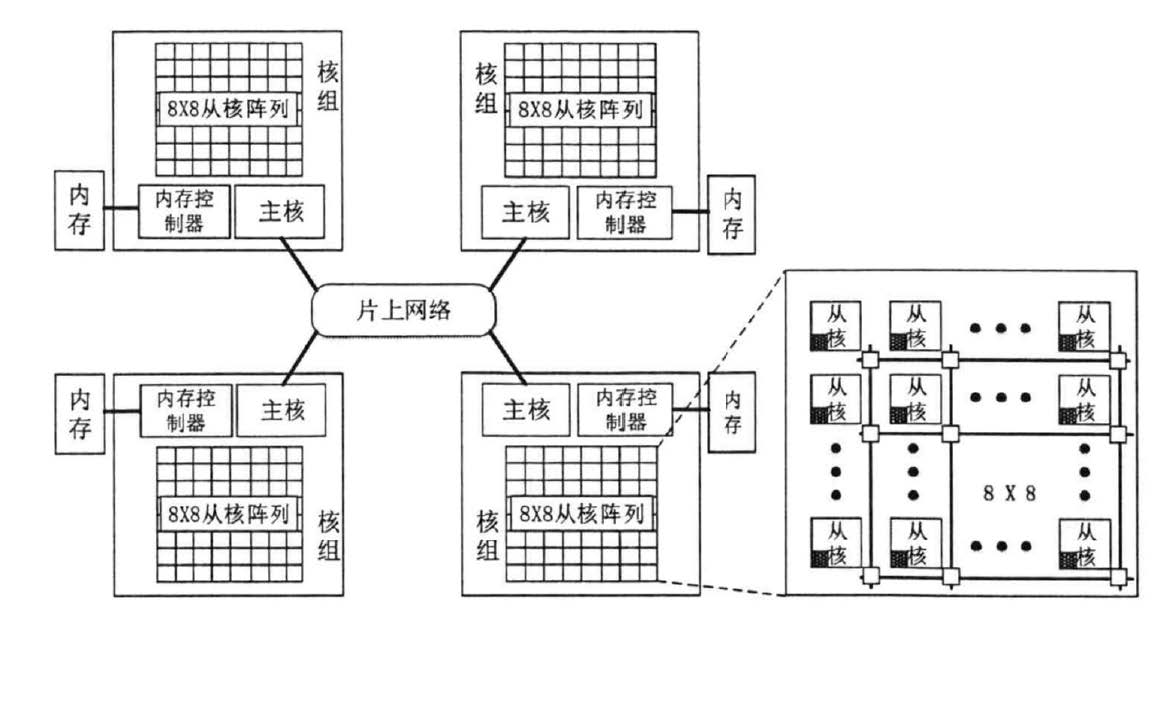
\includegraphics[width=1\textwidth]{1_3.jpg}
  \caption{SW26010 处理器芯片结构图}
\end{figure}

主核和从核都采用了RISC 架构设计,但相对于主核结构,从核得设计和功能较为简单。主核单独访问主存带宽是 9.9GB/s,从核则需要依赖核组接口来完成访存操作,从核阵列最大访存带宽为 30.9GB/s,单个从核最大访存带宽则为10.6GB/s,但受限于总带宽,核组内主从核理论带宽为34GB/s。对于每个主核分别拥有 32KB 的 L1 指令 cache 和 32KB 的 L1 数据 cache,并带有 256KB 的 L2 cache,其中主核访存延迟约为150 个时钟周期。每个从核拥有16KB 的L1 指令cache,而没有数据cache,取而代之的是64KB 的本地存储空间LDM,从核利用DMA 方法进行访问主存的操作的延迟超过 180 个时钟周期,而访问 LDM 的延迟只有数个时钟周期,但与 cache 不同的是 LDM 需要用户手动进行管理,从核在访问主存内的少量数据是,可使用 gld/gst 的方法,每次访问数据块大小不超过 32 字节,对于进行大量数据的读写操作时使用 DMA 方式的性能更好,从核可通过寄存器的方式完成一对多,多对多的通信设计。

对于指令集方面的设计,主核和从核都使用了相同的指令集 SW64 基础指令集,其中有整数运算指令和数据访问指令。但对于浮点指令集的选择和设计,主核和从核之间存在差异,主核的浮点计算指令中的浮点寄存器,是独立于基础寄存器之外的一套寄存器,而从核则是仍然沿用了整数和访存指令中使用的寄存器作为浮点寄存器来使用。对于单指令多数据流SIMD 指令,主核和从核都进行了支持,其中从核支持256 位的向量化运算指令,这种扩展性也为计算提高了精度和性能。除此之外,从核也支持向量混洗指令。在内存管理方面,主存被单独划分为系统内存和应用内存,以减小访存时的冲突行为,系统内存由操作系统进行管理和分配,应用内存则由加载器单独进行管理。

利用DMA 方式进行从核对主存的访问操作通常是高效的,从核在读取主存数据可以利用DMA 方法进行,同时在从核进行数据写回时也可以采用 DMA 方式操作,由于 DMA 本身是以异步方式执行的,从核在进行DMA 操作时并不需要等待执行的完成。DMA 方式并不总是最优的,这是因为 DMA 操作由于读写数据块大小的差异,导致对带宽的使用情况也不尽相同,所以这里我们通过实验分析在DMA 读写数据块尺寸对带宽利用率的影响。表k 表示的是在不同数量从核同时进行DMA 操作时,不同大小数据块对带宽的利用情况。从图中可以看出在利用 64 个从核同时进行读数据时,在数据块达到 128 字节的时候,带宽利用率接近饱和,而当块大小继续增加时,带宽的使用情况保持稳定,在块大小不足 128 字节的时候,带宽利用不够充分。这里也可以根据表中的数据,来选择在使用不同数量的从核进行 DMA 操作时,能够达到最高访存效率的块尺寸。

\paragraph{编程模型}
SW26010 处理器对于用户提供了完备的软件环境支持,其中对于大规模计算的并行也提供了多样化的编程手段。对于节点和核组间的计算并行,用户可选择MPI 方法进行并行,而对于从核阵列上的线程级并行,则可以选择OpenACC添加制导语句或 Athread 线程库的方法进行并行。对于从核级并行的编程方法,最直接方便的是使用 OpenACC 在代码中添加制导语句的方式,OpenACC 编译器会将标记的核心计算放到从核阵列中进行,与此同时进行主从核数据的通信,计算代码的并行等工作。但这种方式与此同时会牺牲性能优化的诸多特特性,包括向量化,寄存器通信等方式,灵活性较低。另外一种方法就是使用Athread 线程库进行从核并行,实际上 OpenACC 编译器就是利用 Athread 线程库来进行的底层实现,利用这种方法同时可以采用从核特性进行深度优化,更加细粒度地处理访存,通信,计算等应用特征。

 \begin{figure}[h]
  \centering
  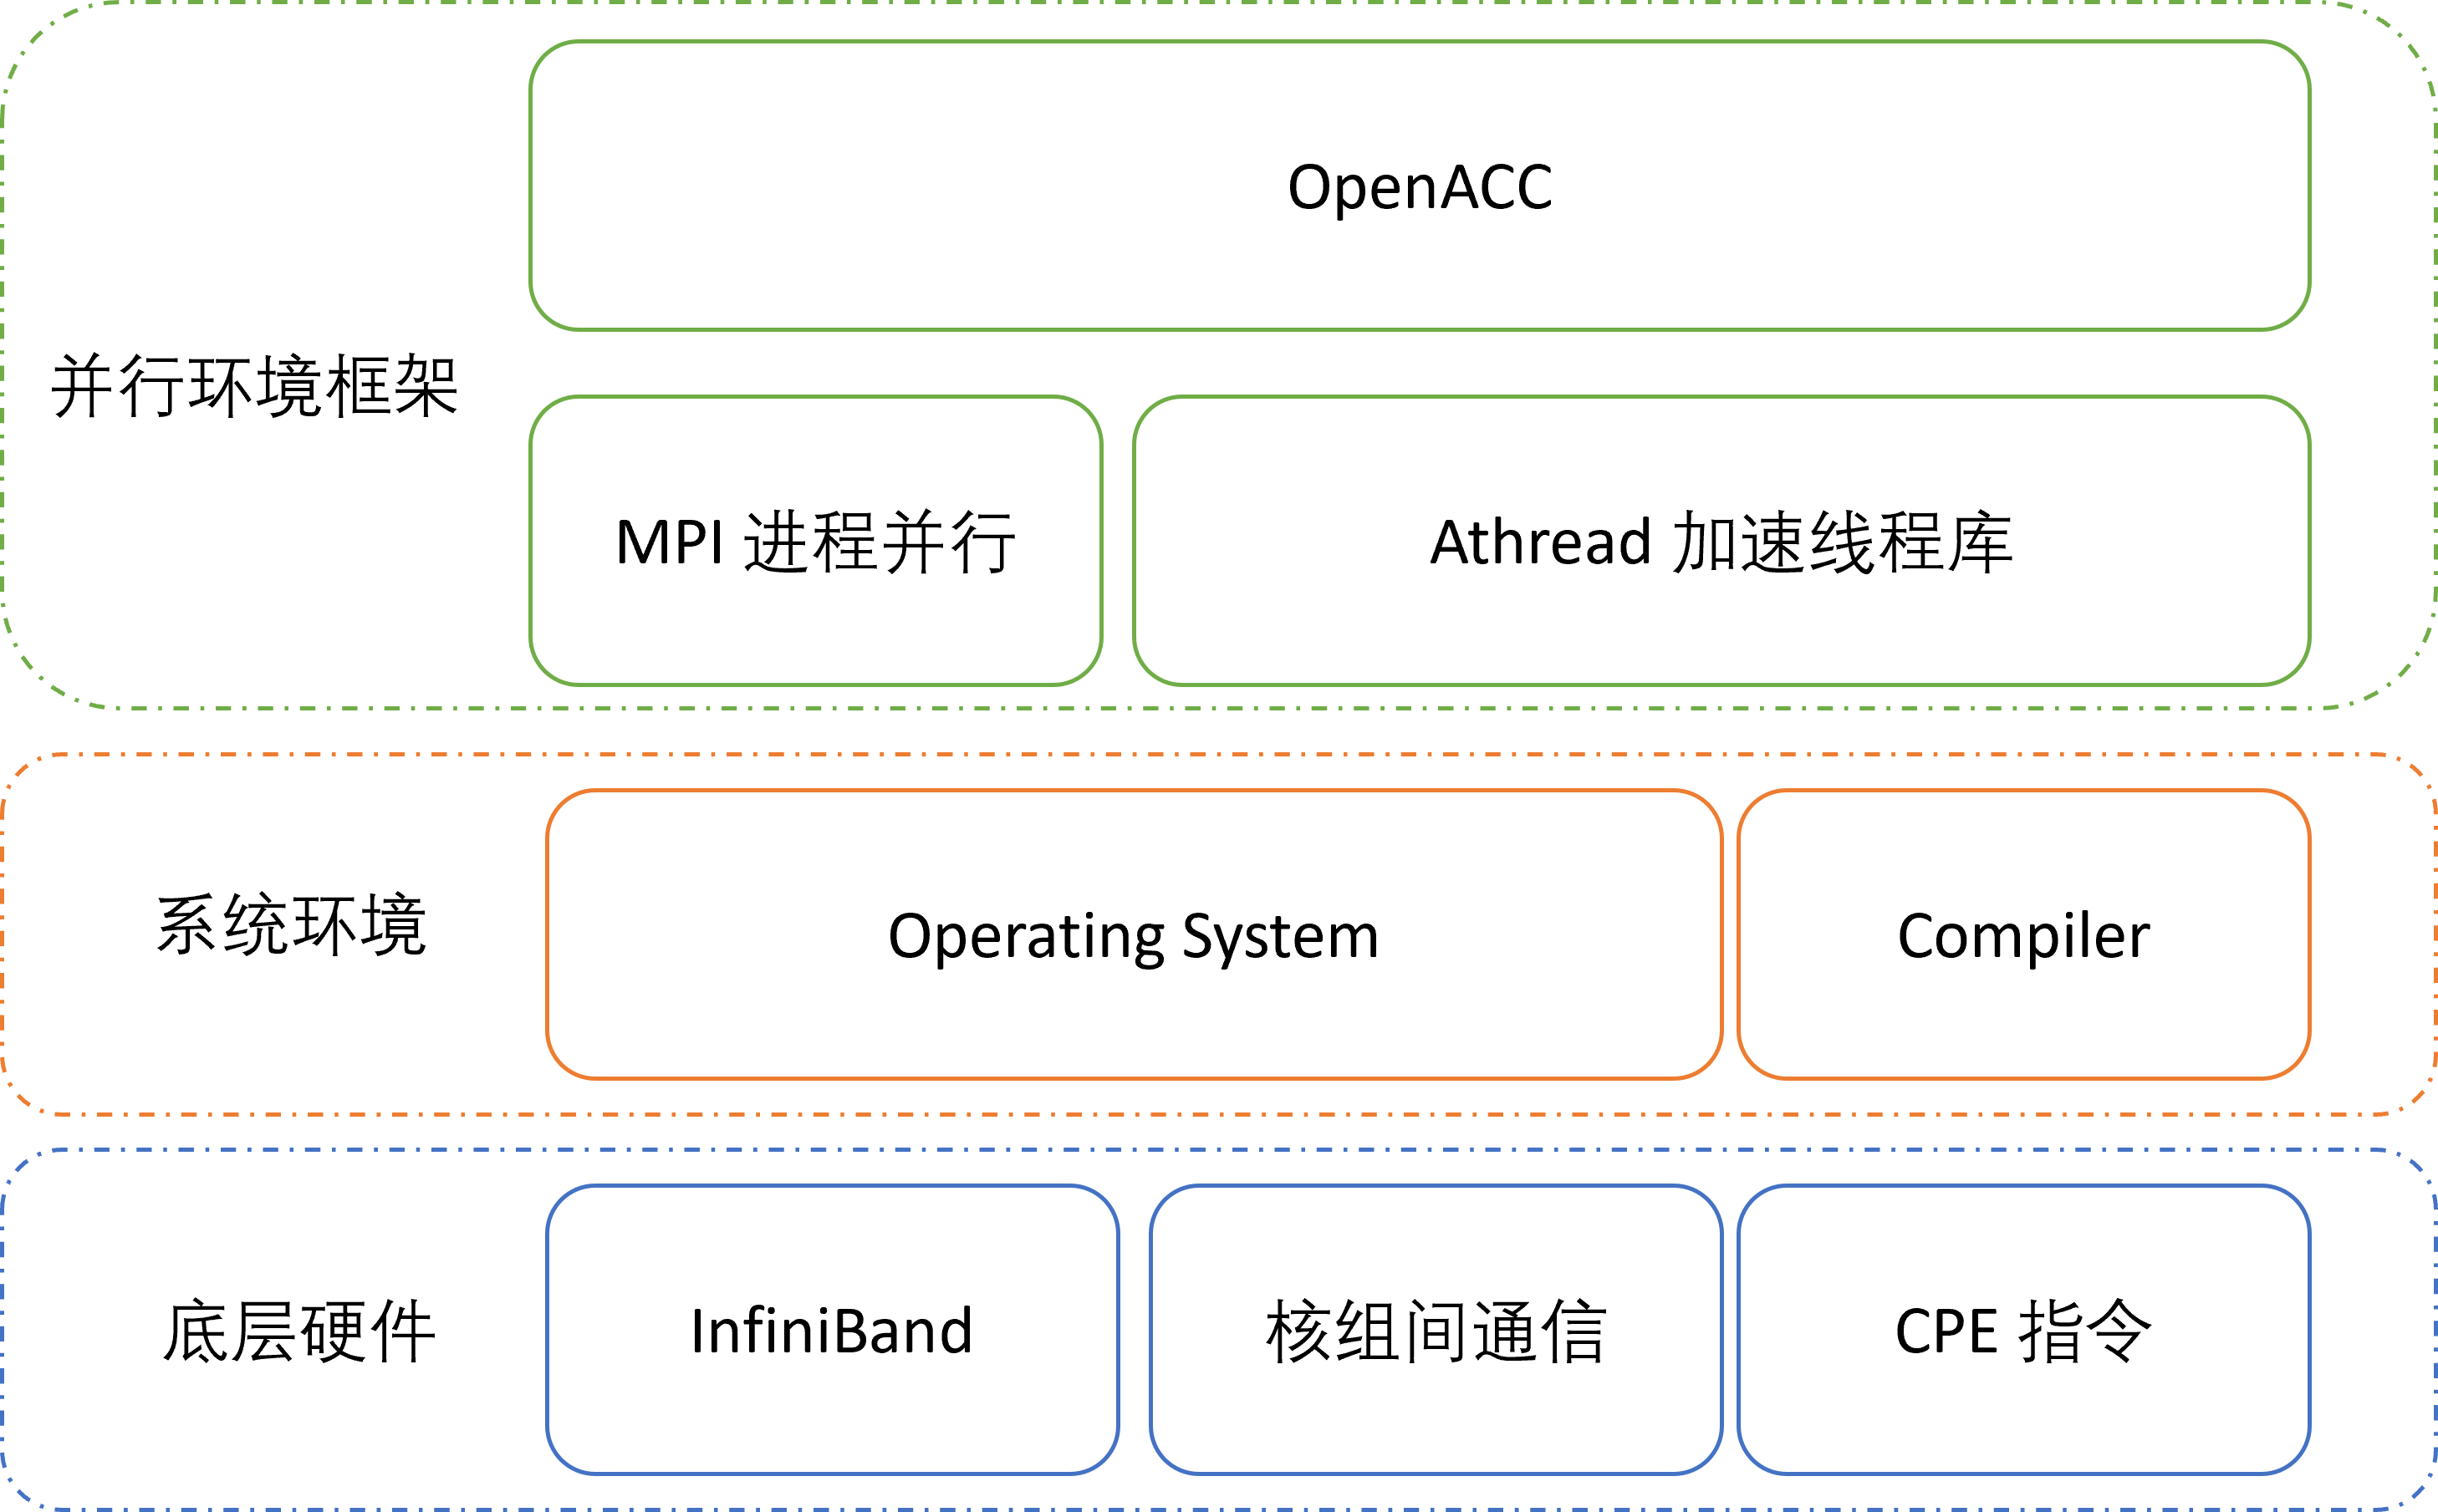
\includegraphics[width=0.7\textwidth]{cpu_level}
  \caption{SW26010 处理器软件库结构}
\end{figure}

\paragraph{并行模式}
对于 SW26010 处理器异构众核的特性,主核主要负责任务调度等控制逻辑方面的任务。与此同时,也可以进行计算任务,而对于从核来说,计算任务负责则是他的主要工作,根据主核和从核的不同任务划分,可分为四种不同的并行模式:
\subparagraph{主从同步模式}
在同步模式中,主核仅设计进程通信,I/O 等串行代码的执行,而完全不参与其中的计算,并行计算任务全部由从核阵列负责,并且在从核进行计算任务时,主核会等待从核任务的完成,不进行任何动作,直到从核将结果返回给主核后,主核才继续执行。这种并行模式方便逻辑简单,并且主核的计算性能远不如整个从核阵列,等待并不会对性能产生大的影响。

\subparagraph{主从协同模式}
在协同模式中,主核除了I/O 操作,数据通信等任务外,还会同时被分配计算任务,与从核同时完成计算负载,并可根据主核与从核计算性能的差异按需分配。在这种模式中,由于主核的参与,计算任务划分得更加均匀,并行度也更高。与此同时也要求不同核心在计算的分配上有着更复杂的控制逻辑。

\subparagraph{主从异步模式}
与主从同步模式类似,主要计算负载仍全部由从核阵列进行,但主核此时则不再进行空等,而是在从核阵列计算的过程中,同时进行部分任务的处理,但不包括核心计算任务部分,例如进行数据通信,I/O 操作等,这样不仅避免了主核参与计算时复杂的控制逻辑,还充分利用了主核的空闲资源。

\subparagraph{主从动态模式}
在此模式中,从核并不会直接获知该轮全部的任务,而是会动态地访问主核,由主核进行任务的动态分配,这样使得计算任务的划分变得不固定。在当从核完成当前分配的计算时,会向主核申请下一阶段的任务。这种模式适合含有大量细粒度任务,且任务之间由很强依赖关系的应用类型。

 \begin{figure}[h]
  \centering
  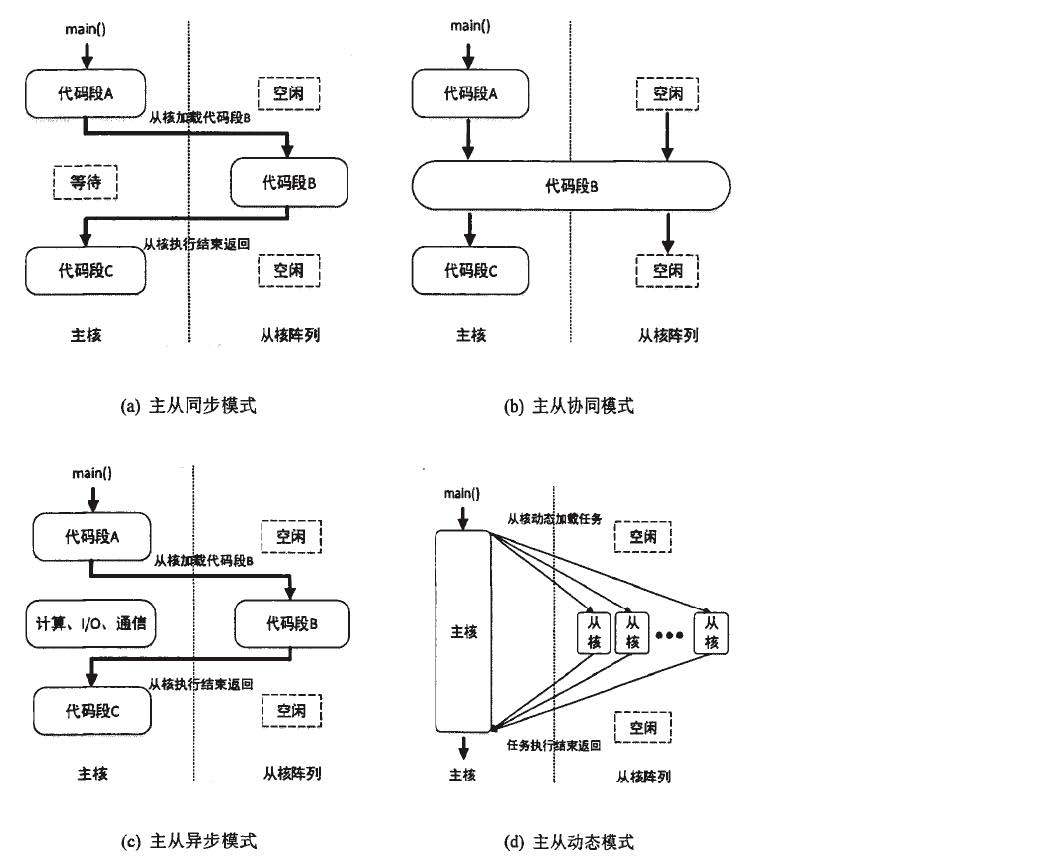
\includegraphics[width=1\textwidth]{1_5.jpg}
  \caption{SW26010 处理器并行模式}
\end{figure}

\section{申威众核平台上应用并行优化面临的挑战}
神威·太湖之光作为世界上计算规模与计算能力都出于前列的超级计算机,上面挂载的 SW26010 异构众核处理器继承了大量的核心计算单元,能够高效进行多类型大规模计算任务的实现。但由于该计算平台架构的特殊性,针对特定类型的计算任务如何能够合理地利用计算资源进行加速才是需要着重关心的问题。首先,与通用平台的计算不同,作为异构众核处理器,无法直接将原来并行化的计算移植到申威平台上,这就要求进行额外并行与优化方案的设计。其次,申威平台上的各类工具均与通用平台差异极大,这里包括编译器的设计,编程语言的支持性,编程接口的调用,外部数学库的支持以及单独的作业与资源管理系统,除此之外,由于平台环境迭代更新较快,软件环境,性能调试工具还不够稳定和完善,且由于平台的特殊性,无法直接参考大多数类型计算的特定优化方案,这就需要在并行优化过程中进行大量的尝试和探索,这无疑会大幅增加工作量。这些问题会为用户在计算并行和性能优化过程中带来极大的挑战。

\subsection{存储结构带来的挑战}
SW26010 处理器中的主核作为通用核心,主要功能是负责计算任务的调度和分配。其核心功能与通用平台处理器核心类似,并且具有FLC 缓存,包括L1指令缓存,L1 数据缓存,也有着L2 缓存区域,但由于每个主核都是相对独立的,所以主核之间并没有共享的 LLC。相对于主要负责任务调度的主核,从核才是进行计算的主要单元,由 8x8 组成的从核阵列与传统的 GPU 计算单元有很大的不同,GPU 计算核心往往使用共享内存空间的方式进行组织,申威处理器上的从核阵列没有任何共享的存储空间,而是对每个从核分配一块独立的地址空间LDM,每个从核独立占用这 64KB 的 LDM,从核之间进行数据通信则必须使用寄存器通信的方式。但这种从核间的寄存器通信方式往往是功能受限的,一是对于从核阵列中的不同核心,不同行列上的从核无法直接进行通信,并且在通信时无法直接获得所传递的数据是来自于哪一个从核上的。因此要想高效利用寄存器通信进行从核间的数据交换,就必须设计一个较为复杂的通信方式,这也要求有更高的调试难度和挑战性。

从核无论以何种方式访问内存,所获得的数据也会被存放在空间受限的LDM 中。而在从核进行计算时,也会优先从LDM 中获取数据,由于LDM 的设计方法,访问LDM 的延迟总是很低,仅有数个时钟周期。这使得将数据优先预取到 LDM,在进行对应从核的计算变成了一种理想的方法,可以大幅减少访存所带来的开销问题。但在实际的计算中这种想法却没办法顺利地实现,这是由于庞大的计算量与有限的存储空间之间的矛盾导致的,在进行分子动力学势函数的计算中,所设计的粒子规模可达数百万,此时对于LDM 来说,每次只能够取到很小一部分数据,这就会导致从核产生较大的访存开销。为了限制访存开销在可接受的范围内,就需要尽可能重用数据,设计出高效的数据存储机制。

\subsection{访存特性带来的挑战}
经测试,SW26010 处理器总访存带宽大小为136GB/s,其中包括4 个核组共260 个核心构成。因此在大量核心同时进行访存操作时,有限的带宽势必会成为阻碍性能的瓶颈。其中从核有两种方式进行访存操作:(1)直接访存方式gld/gst,这种方式通过 cpu 响应中断直接访问主存地址,虽然实现较为容易,但这种方法存在较高延迟的问题,访问单个内存地址需要数百个时钟周期才能完成。(2) DMA 访存方式,利用 DMA 控制器代替相应中断的方式来进行主存访问,在读写大块数据的情况下能够得到较高的性能。但DMA 访存方法存在一些限制,在进行数据访问的时候必须保证地址边界对齐,否则不仅无法提高整体访存效率,还会进一步引发对齐异常的问题。除此之外每次DMA 所读写的数据库大小还会影响整体的访存效率,因为每次进行 DMA 访存时需要进行单独的初始化过程,当读写的数据块大小受限,即使使用DMA 方式读写数据,也无法得到较高的访存效率。由于分子动力学应用有着计算密集的特点,在多个从核同时进行访存时,内存带宽也同样会成为一个问题,此时从核间会有着激烈的带宽竞争,所以如何设计并保证在有限的带宽内进行高效的访存就成为了提高分子动力学计算的重点。

\subsection{指令流水带来的挑战}
SW26010 处理器中只有两条单发射顺序执行流水线,并且每条流水线对应执行不同的指令。第一条流水线负责浮点操作,运行浮点指令。第二天流水线负责访存操作,执行数据移动等指令。所以要想充分利用从核得流水线性能就必须设计合理的计算指令操作。由于从核设计比较简单,不支持乱序执行,且只有基本的分支预测功能,对于除法操作或者开方等超越函数的计算会有更高的延迟。在分子动力学的势函数计算与邻接表索引的过程中,可能出现银寄存器溢出导出的流水线阻塞的问题,因此如何设计多类别混合指令成为了高效利用流水线性能的关键。

 \begin{figure}[h]
  \centering
  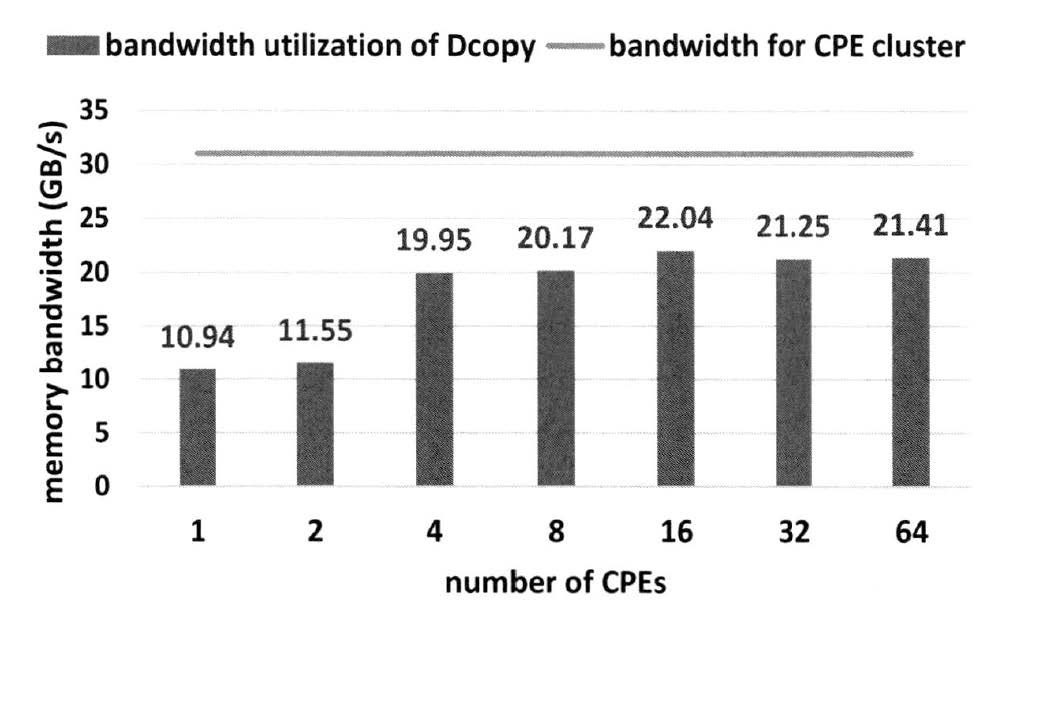
\includegraphics[width=1\textwidth]{1_6.jpg}
  \caption{不同从核数量下DMA速度的变化}
\end{figure}

\section{本文主要研究内容}
本文的主要工作内容是分析分子动力学应用及其特性算法在申威异构众核处理器上的并行实现与计算优化。申威众核平台与其他通用平台不同,自身拥有较强的计算性能,但是却与通用平台有着截然不同的优化方案和策略。并且对于分子动力学以及其他类型的科学应用,优化经验还不够充足。这里主要针对分子动力学软件平台LAMMPS 在神威·太湖之光上的优化方案,对于分子动力学计算,主要涉及多体势基于不同粒子上的计算问题,这也是整体最耗时的部分。除此之外,邻接表的建立和索引,进程间通信和I/O 操作也是优化计算问题的关键。并且为了保证计算的准确性和算法自身高效的性能,还要解决对计算任务的划分,细粒度使用有限的存储空间,并解决并行过程中的读写冲突问题。

本文在实现分子动力学平台LAMMPS 在神威·太湖之光上的移植与优化的同时,在特性计算上根据异构众核的特点也进行了高效的算法设计。在提高分子动力学算法计算性能的同时,也为其他分子动力学软件及科学应用提供了借鉴。文本的研究美容主要分为以下几个方面:

\subsubsection{分子动力学算法的性能分析和并行实现}
为了找到分子动力学算法的核心计算部分,以便接下来进行从核并行与优化,这里首先通过性能分析工具找到热点性能,并分析程序瓶颈,然后整理出热点函数的代码框架,分析程序热点行为,并通过势函数的数据结构,找出计算时的关键信息。将LAMMPS 计算代码移植到主核上进行计算,来确保并行与优化结果的正确性。将计算代码进行改写,由C++ 代码用C 语言进行实现,提出类,虚函数等不支持语言特性,保证计算的兼容性。重构核心计算的数据结构,使得从核计算能够高效进行粒子数据的读写,分析对势函数的计算过程,拆分计算中的迭代部分,完成粒子计算的并行排布,并解决数据依赖和存储空间受限的问题。首先提出内存循环并行的方案,这里的目的是要将核心计算用从核阵列完成,选择对两层粒子迭代的内层进行拆分,也就是根据邻接表对每个中心粒子对应的邻居粒子计算均匀分配到 64 个从核上进行,并且保证在同一个周期内单个从核的计算量基本相同,针对在划分后出现的数据依赖问题,也通过在从核阵列上选择特性的从核进行数据归约的办法来解决。然后又设计了副本归约的方法来完成粒子计算,这种方法选择了对外层迭代进行拆分,进一步提高了计算的并行度和计算效率,这种方法利用从核LDM 上的空间来暂存该时间步内当前从核所计算的结果,并在该轮计算全部完成后,由指定从核进行数据的累加,将结果写回主存。

\subsubsection{分子动力学算法的优化方案}
对于从核计算时受力信息的累加,设计了高效的从核通信归约方法。这里由于从核间采用了寄存器的方法进行通信,而这种方法只能在同行列的从核之间进行数据交换,所以这种利用了一种基于二叉树的设计方案,分别将数据写入到行首和列首,来得到最终累加的结果,与此同时还利用从核同步解决了由归约次序不同造成的结果混乱的问题。文本还设计了一种单端更新的方案,这种方法通过平衡算法中的计算量,来换取更好而访存性能,并且占用更小的从核LDM 空间,通过修改邻接表的方法,使得通过少量的冗余计算提高算法的整体性能,并且支持在更大规模体系下的计算模拟。另外,通过中计算过程的分析,这里将计算热点的常用数据预取到从核LDM 中,使其在当前时间步的计算内能够被快速访问,从核降低访存开销。这里也通过手动DMA 操作将大块的粒子信息读到从核存储空间内,来进一步提升性能。

为了充分利用粒子数据的就是局部性,合理地完成数据的重用,设计了高效的从核软件 cache,通过分析从核 LDM 空间,完成针对分子动力学特定算法的数据替换和重用。并且结合 DMA 访存策略,能够在软件 cache 中得到很高的数据命中率,并且算法中粒子的计算采用了合适的向量化方案,依靠向量混洗完成离散粒子数据的读取,进一步提高了算法的整体性能。

\section{论文结构}
本文共有六个章节,对应结构如下:

第一章是绪论,简单介绍了分子动力学算法的发展,经典算法的研究背景,对多核计算机处理器进行简述,并给出了对于申威平台上分子动力学计算的核心挑战,最后是本文的主要工作内容。

第二章为相关工作,给出了分子动力学中 eFF 算法的描述,LAMMPS 分子动力学平台的简述以及 LAMMPS 在当前不同硬件架构和计算上的并行实现。

第三章给出了eFF 算法在神威·太湖之光上的热点函数分析,以及LAMMPS计算的基本移植,接下来通过对核心数据和任务划分的分析,设计了两种不同的并行方案,并给出这两种方案所采用的划分策略。

第四章根据神威·太湖之光上各类优化方案,分别从通信,计算,访存等多个方面进行eFF 算法的优化,并给出了一种是适配性更强,性能方面更优秀的并行方案,通过堆势函数计算部分的分析,消除了LAMMPS 计算在申威平台上所遇到的瓶颈问题。

第五章是本文的实验与性能分析部分,通过完备详尽的实验和测试,给出了对于 LAMMPS 计算在不同优化策略和并行方案上的具体表现。

第六章是全文总结,对文本的研究工作和优化方案进行回顾和总结,并给出未来相关工作的方向。

